\documentclass{article}
\usepackage{mathtools}
\usepackage{amssymb}
\usepackage{listings,xcolor}
\usepackage{physics}

\lstset{language=Mathematica}
\lstset{basicstyle={\sffamily\footnotesize},
  numbers=left,
  numberstyle=\tiny\color{gray},
  numbersep=5pt,
  breaklines=true,
  captionpos={t},
  frame={lines},
  rulecolor=\color{black},
  framerule=0.5pt,
  columns=flexible,
  tabsize=2
}

\begin{document}
\title{On the Distribution of $Z\sim\chi^2_{df} + \text{Lap}(b)$}
\author{Mark Schultz}
\maketitle
\section{Background}
When discussion a differentially private form of ANOVA, we looked into the following random variable:
\begin{equation}
\widehat{F}\sim \frac{U_1+\text{Lap}(b_1)}{U_2+\text{Lap}(b_2)}
\end{equation}
Here, $U_1$ and $U_2$ are both $\chi^2_{df}$ for some parameter $df$.
The first step to understanding this random variable would be understanding the distribution of $U+\text{Lap}(b)$ for $U\sim\chi^2_{df}$.
Does this potentially have a ``nice'' distribution?
\section{Computing the PDF via Mathematica}
We can attempt to answer this question via Mathematica, which has a ``Transform Distribution'' function.
Utilizing this, we can find the pdf $\rho_{X+Y}(x)$:
\begin{center}
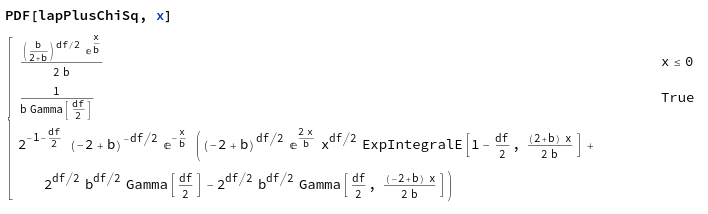
\includegraphics[scale=.5]{pdf.png}
\end{center}
The pdf is piecewise defined, on the regions $x \leq 0$, and $x > 0$.
When $x \leq 0$, it follows that:
\begin{equation}
\rho_{X+Y}(x) = \frac{b^{(df/2)-1}}{2(b+2)^{df/2}}e^{x/b}
\end{equation}
The region $x > 0$ is more complicated.
Here, we have that:
\begin{align*}
\rho_{X+Y}(x) &=\frac{e^{-x/b}}{\Gamma(df/2)2^{(df/2)+1}(b-2)^{df/2}b}\left(-2^{df/2}b^{df/2}\Gamma\pqty{df/2,\frac{(b-2)}{2b}x} + 2^{df/2}b^{df/2}\Gamma(df/2)\right. \\
&+\left.(b-2)^{df/2}e^{2x/b}x^{df/2}E_{1-(df/2)}\pqty{\frac{(b+2)}{2b}x}\right)
\end{align*}
Note here that the first two terms can be rewritten as:
\begin{equation}
2^{df/2}b^{df/2}\pqty{\Gamma(df/2)-\Gamma\pqty{df/2, \frac{(b-2)}{2b}x}}
\end{equation}
Here, we have that:
\begin{equation}
\Gamma(a) = \int_0^\infty x^{a-1}e^{-x}\mathrm{ d}x
\end{equation}
is the \emph{Gamma function}.
This has two related functions defined, the \emph{upper} and \emph{lower} incomplete Gamma functions:
\begin{equation}
\Gamma(a,b) = \int_b^\infty x^{a-1}e^{-x}\mathrm{d}x,\quad \gamma(a,b) = \int_0^b x^{a-1}e^{-x}\mathrm{d}x
\end{equation}
These satisfy:
\begin{equation}
\gamma(a,b) + \Gamma(a,b) = \Gamma(a)\implies \Gamma(a) - \Gamma(a,b) = \gamma(a,b)
\end{equation}
It follows that the aforementioned term is just:
\begin{equation}
(2b)^{df/2}\gamma\pqty{df/2, \frac{(b-2)}{2b} x}
\end{equation}
It follows that the pdf is (in the region $x > 0$):
\begin{align*}
\frac{e^{-x/b}}{\Gamma(df/2)2^{(df/2)+1}(b-2)^{df/2}b}\pqty{(2b)^{df/2}\gamma\pqty{df/2,\frac{(b-2)}{2b}x} + (b-2)^{df/2}e^{2x/b}x^{df/2}E_{1-(df/2)}\pqty{\frac{(b+2)}{2b}x}}
\end{align*}
Here, $E_{n}(a)$ is (a generalization of) the \emph{exponential integral}, and can be written as:
\begin{equation}
E_{n}(x) = \int_1^\infty \frac{e^{-xt}}{t^n}\mathrm{d}t
\end{equation}
This can be seen as a special case of the (upper) incomplete gamma function.
Specifically:
\begin{equation}
E_n(x) = x^{n-1}\Gamma(1-n,x)
\end{equation}
It follows that:
\begin{equation}
E_{1-(df/2)}\pqty{\frac{(b+2)}{2b}x} = \pqty{\frac{(b+2)}{2b}x}^{-df/2}\Gamma\pqty{df/2,\frac{(b+2)}{2b}x}
\end{equation}
Examining the rest of that term, we see that it's equal to:
\begin{equation}
\pqty{\frac{b-2}{b+2}}^{df/2}e^{2x/b}(2b)^{df/2}\Gamma\pqty{df/2,\frac{(b+2)}{2b}x}
\end{equation}
Now, it follows that the pdf is:
\begin{equation}
\frac{1}{2b\Gamma(df/2)}\pqty{\pqty{\frac{b}{b-2}}^{df/2}e^{-x/b}\gamma\pqty{df/2,\frac{(b-2)}{2}(x/b)} + \pqty{\frac{b}{b+2}}^{df/2}e^{x/b}\Gamma\pqty{df/2,\frac{(b+2)}{2}(x/b)}}
\end{equation}
This could also be written in terms of the \emph{regularized incomplete gamma functions}, which are defined as:
\begin{equation}
P(a,b) = \frac{\gamma(a,b)}{\Gamma(a)},\quad Q(a,b) = \frac{\Gamma(a,b)}{\Gamma(a)}
\end{equation}
At this time, I see no gain by doing this, although if we wanted to implement this later it's possible\footnote{I'm unsure how a computer algebra system typically computes this quantities, but if it's via a series approximation I'd imagine that the series for $P(a,b)$ and $Q(a,b)$ would be more efficient, provided they exist.} that computing $P(a,b)$ is both more efficient, and more accurate than computing $\frac{\gamma(a,b)}{\Gamma(a)}$.

With this, we can write down the entire pdf of $Z\sim \chi^2_{df} + \text{Lap}(b)$.
\begin{align*}
\rho_Z(x) = \begin{cases} \frac{1}{2b}\pqty{\frac{b}{b+2}}^{df/2}e^{x/b} & x \leq 0 \\
\frac{1}{2b}\pqty{\pqty{\frac{b}{b+2}}^{df/2}e^{x/b}\frac{\Gamma\pqty{df/2,\frac{(b+2)}{2}(x/b)}}{\Gamma(df/2)} + \pqty{\frac{b}{b-2}}^{df/2}e^{-x/b}\frac{\gamma\pqty{df/2,\frac{(b-2)}{2}(x/b)}}{\Gamma(df/2)}} & x > 0
\end{cases}
\end{align*}
\subsection{Deriving the PDF: A Sketch}
While I won't derive the PDF right now (as it only seems worthwhile to do if we want to publish it, and don't want to cite Mathematica), I can imagine the following technique would work quite well.

Let $X\sim\text{Lap}(b)$, and $Y\sim\chi^2_{df}$.
Then:
\begin{equation}
\rho_X(x) = \frac{1}{2b}e^{-\abs{x}/b},\quad \rho_Y(y) = \frac{1}{2^{df/2}\Gamma(df/2)}y^{df/2-1}e^{-y/2}
\end{equation}
The pdf for $Z\sim X+Y$ with $X,Y$ independent can be written down as\footnote{$\rho_X$ is chosen to be the function with argument $t$ instead of $z - t$, as it makes working with the absolute value easier.
This doesn't \emph{really} matter, as we can always use a $u$-substitution later.}:
\begin{equation}
\rho_Z(z) = \int_{t = -\infty}^\infty \rho_X(t)\rho_Y(z-t)\mathrm{d}t
\end{equation}
Note that this assumes that $\rho_X$ and $\rho_Y$ have the same domain.
In our case, we have that:
\begin{equation}
\mathbb{R} = \text{dom}(\rho_X) \neq \text{dom}(\rho_Y) = [0,\infty)
\end{equation}
One way to change that is to write:
\begin{equation}
\rho_Y(y) = \frac{1}{2^{df/2}\Gamma(df/2)}y^{df/2-1}e^{-y/2}\chi_{[0,\infty)}(y)
\end{equation}
Now, they have the same domain, so convolving them makes sense.
We then have that:
\begin{align*}
\rho_Z(z) &= \frac{1}{(2b)2^{df/2}\Gamma(df/2)}\int_{t = -\infty}^\infty e^{-\abs{t}/b} (z-t)^{(df/2)-1}e^{-(z-t)/2}\chi_{[0,\infty)}(z-t)\mathrm{d}t
\end{align*}
We then would:
\begin{enumerate}
\item Split the integral into $\int_{-\infty}^0 + \int_0^\infty$ to deal with the absolute value.
\item Make the substitution $u = z-t$ to deal with the annoying stuff\footnote{Specifically, this will mean we're working with $\rho_Y(u)$ instead of $\rho_Y(z-t)$, which is the ``annoying stuff''.} left over.
\item Incorporate the $\chi_{[0,\infty)}(z-t)$ into the bounds\footnote{This is by the trick that $\int_{-\infty}^\infty f(x)\chi_{[a,b]}(x)\mathrm{d}x = \int_a^b f(x)\mathrm{d}x$.}.
\item Finish integrating things, and anticipate being ``stuck'' on some integrals, which will be written as incomplete Gamma functions.
\end{enumerate}
None of this seems difficult, just tedious, and unnecessary until (potentially) later on.
\section{The Ratio Distribution}
In addition to the above, given random variables $X,Y$ that are independent, there is a general way to compute the distribution of $Z\sim X/Y$ (known as the \emph{ratio distribution}).
This can be done easily via our normal method of passing through the CDF, and gives the final result:
\begin{equation}
\rho_Z(z) = \int_{y = -\infty}^\infty\abs{y} \rho_{X,Y}(zy,y)\mathrm{ d}y = \int_{y = -\infty}^\infty \abs{y}\rho_X(zy)\rho_Y(y)\mathrm{ d}y
\end{equation}
It seems unlikely we'll be able to compute this for $X,Y\sim\chi^2_{df} + \text{Lap}(b)$.
It would be a great deal of work due to $\rho_X(x)$ being piecewise defined.
We would need to split up the overall integral into:
\begin{align*}
\int_{y =-\infty}^0 (-y)\rho_X(zy)\rho_Y(y)\mathrm{d}y + \int_{y =0}^\infty y\rho_X(zy)\rho_Y(y)\mathrm{d}y
\end{align*}
Each of these would need to be evaluated separately for $z \leq 0$ and $z > 0$.
As $\rho_X$ and $\rho_Y$ are distributed the same\footnote{This isn't really true, as each will have (potentially separate) parameters $(b_x,df_x)$ and $(b_y,df_y)$.
Still, a special case of this will be the parameters being identical.
We can try to examine this (easier) case, and notice that it still seems not possible.}, we will just write $\rho$.
We can then write $\rho_{\leq 0}(x)$ for the part of the piecewise function defined on the region $\mathbb{R}_{\leq 0}$, and $\rho_{>0}(x)$ for the other part.

We can then see we'll have to compute \emph{four} integrals, as each of the above two will have two separate cases when $z \leq 0$, and $z > 0$.
To see how bad it can really get, we can examine the \emph{worst} integral, which should be:
\begin{equation}
\int_{y = 0}^\infty y\rho_{>0}(zy)\rho_{>0}(y)\mathrm{d}y,\quad z > 0
\end{equation}
This will end up being four terms\footnote{This is just because it'll be $\int (a+b)(c+d) = \int ac + \int ad + \int bc + \int bd$.}, the first of which will be:
\begin{equation}
\frac{1}{(2b)^2\Gamma(df/2)^2}\pqty{\frac{b}{b+2}}^{df}\int_{y = 0}^\infty\pqty{e^{y(z+1)/b}\pqty{\int_{t = \frac{b+2}{2}(yz/b)}^{\infty}t^{(df/2)-1}e^{-t}\mathrm{d}t}\pqty{\int_{t = \frac{b+2}{2}(y/b)}^{\infty}t^{(df/2)-1}e^{-t}\mathrm{d}t}}
\end{equation}
Completing this integration quite difficult.
Fortunately, I believe the other 15 terms would be easier, but I doubt by that much.

Additionally, Mathematica fails to compute a closed form of the PDF, despite working for $\chi^2_{df}+\text{Lap}(b)$.
This failure even occurs in the ``easy'' case, when $X$ and $Y$ have the same parameters $(b_x,df_x) = (b_y,df_y)$.
\end{document}